\documentclass{report}
\usepackage{Custom_Latex/Summary_Notes/notes}
\addtolength{\oddsidemargin}{-.5in}
\addtolength{\evensidemargin}{-.5in}
\addtolength{\textwidth}{1in}
\usepackage{import}
\usepackage{graphicx}
\usepackage{pgf}
\usepackage{printlen}
\usepackage{wrapfig}

\begin{document}
\title{IADS - CW 2}
\author{Maksymilian Mozolewski}
\maketitle
\pagebreak
\section{Task1}

\subsection*{Q 1.2}
After estimating and saving the covariance/correlation matrices i plotted them in matplotlib as a heat map, which can be seen below:
\begin{figure}[h]
    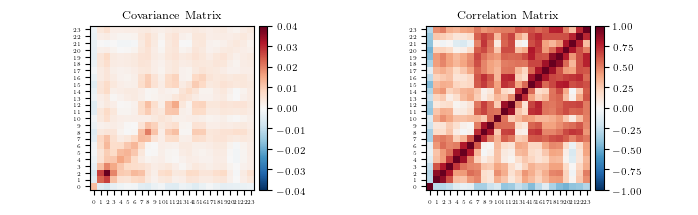
\includegraphics[scale=1,left]{Years/Year2/Semester2/Learning/CW/python_code/correlation.png} 
    \caption{Heatmaps for the covariance and correlation matrices}
\end{figure}
After looking at the graph, the fist thing that stands out is that the 0th variable is negatively correlated with most of the other variables, and that the only other variable pairs with negative correlations are: 21 and 3,21 and 4,21 and 2. there are quite many variables with strong positive correlations mostly near the diagonal but also spread around the graph. Variables to the left of the 7th column, are more weakly correlated with all the rest, than the ones to the right. Looking at just the covariance matrix i can also see that variables 2,3,4 have much higher variance than the rest.
\subsection*{Q 1.3}
{
    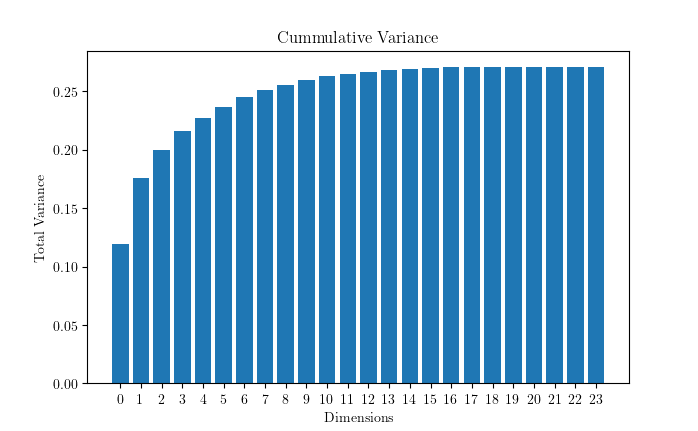
\includegraphics{Years/Year2/Semester2/Learning/CW/python_code/cumvar.png}
    \caption{Figure 2: A graph of the cummulative variance of eigenvalues from the dataset}
}
\end{document}